
\documentclass[11pt]{beamer}
%Packages
\usepackage{multirow}
\usepackage{graphicx}
\usepackage[utf8x]{inputenc}
\usepackage[T1]{fontenc}
\usepackage{aeguill}
\usepackage{amssymb}
\usepackage{pgf,pgfarrows,pgfnodes}
\usepackage[french]{babel}
\usepackage{float}
\usepackage{xkeyval,calc,listings,tikz}
\usepackage{slashbox}
\usepackage{fancyvrb}

%Preamble

\input /Users/remy/cqls/texinputs/Cours/cqlsInclude
\input /Users/remy/cqls/texinputs/Cours/testInclude


\mode<article>{\usepackage{fullpage}}
%\usetheme{Darmstadt}
%\usepackage{times}
%\usefonttheme{structurebold}
\usetheme{Antibes}
%\usecolortheme{lily}

\definecolor{VertFonce}{rgb}{0,.4,.0}

\mode<presentation>
{
  %\usetheme{Warsaw}
  % or ...
\usetheme{Boadilla}

  \setbeamercovered{transparent=5}
  % or whatever (possibly just delete it)
}
%\setbeamercovered{dynamic}


\subject{Talks}

\AtBeginSection[]
{
  \begin{frame}<beamer>
    \frametitle{Plan}
    \tableofcontents[currentsection,currentsubsection]
  \end{frame}
}


\setbeamercovered{invisible}
\newcommand{\Sim}{{\star}}
\newcommand{\ok}{ \textcolor{green}{\large$\surd$}}
\newcommand{\nok}{ \textcolor{red}{\large X}}


\usetikzlibrary{arrows,%
  calc,%
  fit,%
  patterns,%
  plotmarks,%
  shapes.geometric,%
  shapes.misc,%
  shapes.symbols,%
  shapes.arrows,%
  shapes.callouts,%
  shapes.multipart,%
  shapes.gates.logic.US,%
  shapes.gates.logic.IEC,%
  er,%
  automata,%
  backgrounds,%
  chains,%
  topaths,%
  trees,%
  petri,%
  mindmap,%
  matrix,%
  calendar,%
  folding,%
  fadings,%
  through,%
  positioning,%
  scopes,%
  decorations.fractals,%
  decorations.shapes,%
  decorations.text,%
  decorations.pathmorphing,%
  decorations.pathreplacing,%
  decorations.footprints,%
  decorations.markings,%
  shadows}
\tikzset{
  every plot/.style={prefix=plots/pgf-},
  shape example/.style={
    color=black!30,
    draw,
    fill=yellow!30,
    line width=.5cm,
    inner xsep=2.5cm,
    inner ysep=0.5cm}
}

\definecolor{darkgreen}{rgb}{0,.4,.0}

%Styles

%Title

\beamertemplateshadingbackground{green!50}{yellow!50}
\title[Problématiques Produits A et B]
{Cours de Statistiques Inférentielles}
\author{CQLS~: cqls@upmf-grenoble.fr}
\date{\today}

\begin{document}
\maketitle


%\begin{frame}
%  \titlepage
%\end{frame}

\section{Exemples de comparaisons de paramètres}
\begin{frame}
\frametitle{Objectif et questions}

\begin{exampleblock}{Problématique associée à ce cours}
On s'intéresse aux performances relatives de l'ensemble des petites et moyennes entreprises (PME) de deux pays fictifs notés P1 et P2 en 2004 et 2005 en analysant leurs chiffres d'affaires (exprimés dans une même unité). Ne pouvant pas interroger l'ensemble des PME, on ne pourra disposer que des chiffres d'affaires sur des échantillons de PME (les tailles d'échantillons seront précisées plus tard).
\end{exampleblock}


\begin{block}{Question 1}
En 2005, le C.A. annuel moyen des PME du pays $P_1$ est-il de plus de 20 unités supérieur à celui du pays $P_2$~?
\end{block}

\begin{block}{Question 2}
En 2005, le C.A. annuel moyen des PME du pays $P_1$ est-il de plus de 20\% supérieur à celui du pays $P_2$~?
\end{block}

\begin{tikzpicture}[remember picture,overlay]
  \node [rotate=30,scale=10,text opacity=0.05]
    at (current page.center) {CQLS};
\end{tikzpicture}\end{frame}

\begin{frame}
\frametitle{Questions (suite)}


\begin{block}{Question 3}
En 2005, l'hétérogénéité (mesurée par la variance) des C.A. annuels des PME du pays $P_1$ est-elle différente de celle du pays $P_2$~?
\end{block}
 
\begin{block}{Question 4}
En 2005, l'hétérogénéité des C.A. annuels des PME du pays $P_1$ est-elle de plus de 25\% supérieure à celle du pays $P_2$~?
\end{block}

\begin{block}{Question 5}
{\small Le C.A. moyen des PME de P1 a-t-il augmenté de plus de 10 unités entre 2004 et 2005~?
Pour traiter cette question, on disposera des chiffres d'affaires des mêmes $n$ PME en 2004 et 2005.}
\end{block}
\begin{tikzpicture}[remember picture,overlay]
  \node [rotate=30,scale=10,text opacity=0.05]
    at (current page.center) {CQLS};
\end{tikzpicture}\end{frame}

\section{Problématiques avec 2 paramètres}
\begin{frame}

\begin{pgfpicture}{0cm}{0cm}{11cm}{8cm}
\pgfsetendarrow{\pgfarrowto}
\pgfnodebox{CritInt}[stroke]{\pgfxy(5.5,8)}{\color[rgb]{0,0,1}Nbre de paramètres pour décrire $\mathbf{H_1}$~?}{2pt}{2pt}
\pgfnodebox{Par1}[stroke]{\pgfxy(3.5,6.4)}{1 paramètre}{2pt}{2pt}
\pgfnodeconncurve{CritInt}{Par1}{-90}{90}{0.5cm}{0.5cm}
\pgfnodebox{Par2}[stroke]{\pgfxy(7.5,7.2)}{2 paramètres}{2pt}{2pt}
\pgfnodeconncurve{CritInt}{Par2}{-90}{90}{0.5cm}{0.5cm}

\end{pgfpicture}
\pgftext[top,right,at={\pgfxy(0,4.0)}]{\begin{minipage}{11cm}


\end{minipage}}

\end{frame}

\begin{frame}

\begin{pgfpicture}{0cm}{0cm}{11cm}{8cm}
\pgfsetendarrow{\pgfarrowto}
\pgfnodebox{CritInt}[stroke]{\pgfxy(5.5,8)}{\color[rgb]{0,0,1}Nbre de paramètres pour décrire $\mathbf{H_1}$~?}{2pt}{2pt}
\pgfnodebox{Par2}[stroke]{\pgfxy(7.5,7.2)}{2 paramètres}{2pt}{2pt}
\pgfnodeconncurve{CritInt}{Par2}{-90}{90}{0.5cm}{0.5cm}

\end{pgfpicture}
\pgftext[top,right,at={\pgfxy(0,4.0)}]{\begin{minipage}{11cm}


\end{minipage}}

\end{frame}

\begin{frame}

\begin{pgfpicture}{0cm}{0cm}{11cm}{8cm}
\pgfsetendarrow{\pgfarrowto}
\pgfnodebox{CritInt}[stroke]{\pgfxy(5.5,8)}{\color[rgb]{0,0,1}Nbre de paramètres pour décrire $\mathbf{H_1}$~?}{2pt}{2pt}
\pgfnodebox{Par2}[stroke]{\pgfxy(7.5,7.2)}{2 paramètres}{2pt}{2pt}
\pgfnodeconncurve{CritInt}{Par2}{-90}{90}{0.5cm}{0.5cm}
\pgfnodebox{CritEch}[stroke]{\pgfxy(7.5,6.4)}{\color[rgb]{0,0,1}Nbre d'échantillons~?}{2pt}{2pt}
 \pgfnodeconncurve{Par2}{CritEch}{-90}{90}{0.5cm}{0.5cm}

\end{pgfpicture}
\pgftext[top,right,at={\pgfxy(0,4.0)}]{\begin{minipage}{11cm}


\end{minipage}}

\end{frame}

\begin{frame}

\begin{pgfpicture}{0cm}{0cm}{11cm}{8cm}
\pgfsetendarrow{\pgfarrowto}
\pgfnodebox{CritInt}[stroke]{\pgfxy(5.5,8)}{\color[rgb]{0,0,1}Nbre de paramètres pour décrire $\mathbf{H_1}$~?}{2pt}{2pt}
\pgfnodebox{Par2}[stroke]{\pgfxy(7.5,7.2)}{2 paramètres}{2pt}{2pt}
\pgfnodeconncurve{CritInt}{Par2}{-90}{90}{0.5cm}{0.5cm}
\pgfnodebox{CritEch}[stroke]{\pgfxy(7.5,6.4)}{\color[rgb]{0,0,1}Nbre d'échantillons~?}{2pt}{2pt}
 \pgfnodeconncurve{Par2}{CritEch}{-90}{90}{0.5cm}{0.5cm}
\pgfnodebox{Ech1}[stroke]{\pgfxy(6,5.6)}{1 échantillon}{2pt}{2pt}
 \pgfnodeconncurve{CritEch}{Ech1}{-90}{90}{0.5cm}{0.5cm}

\end{pgfpicture}
\pgftext[top,right,at={\pgfxy(0,4.0)}]{\begin{minipage}{11cm}


\end{minipage}}

\end{frame}

\begin{frame}

\begin{pgfpicture}{0cm}{0cm}{11cm}{8cm}
\pgfsetendarrow{\pgfarrowto}
\pgfnodebox{CritInt}[stroke]{\pgfxy(5.5,8)}{\color[rgb]{0,0,1}Nbre de paramètres pour décrire $\mathbf{H_1}$~?}{2pt}{2pt}
\pgfnodebox{Par2}[stroke]{\pgfxy(7.5,7.2)}{2 paramètres}{2pt}{2pt}
\pgfnodeconncurve{CritInt}{Par2}{-90}{90}{0.5cm}{0.5cm}
\pgfnodebox{CritEch}[stroke]{\pgfxy(7.5,6.4)}{\color[rgb]{0,0,1}Nbre d'échantillons~?}{2pt}{2pt}
 \pgfnodeconncurve{Par2}{CritEch}{-90}{90}{0.5cm}{0.5cm}
\pgfnodebox{Ech1}[stroke]{\pgfxy(6,5.6)}{1 échantillon}{2pt}{2pt}
 \pgfnodeconncurve{CritEch}{Ech1}{-90}{90}{0.5cm}{0.5cm}

  \pgfnodebox{Asympt}[stroke]{\pgfxy(3,4.4)}{\color[rgb]{0,0.6,0}Asymptotique}{2pt}{2pt}
\pgfnodeconncurve{Ech1}{Asympt}{-90}{90}{0.5cm}{0.5cm}
\pgfnodebox{Par1}[stroke]{\pgfxy(3.5,6.4)}{1 paramètre}{2pt}{2pt}
\pgfnodeconncurve{CritInt}{Par1}{-90}{90}{0.5cm}{0.5cm}
\pgfnodeconncurve{Par1}{Asympt}{-90}{90}{0.5cm}{0.5cm}

\end{pgfpicture}
\pgftext[top,right,at={\pgfxy(0,4.0)}]{\begin{minipage}{11cm}
\hrulefill\\
%%% 2 params, 1 ech et asympt et %%% 2 params, 1 ech et gaussien
\noindent \textbf{Paramètre~:} $\mu^{(1)}-\mu^{(2)}=\mu^D:=\EEE{Y^D_i}$={\color{purple}``moyenne de Différence"}\\
où $Y^D_i:=Y^{(1)}_i-Y^{(2)}_i$={\color{purple}``Différence de variables"}\\
\noindent\textbf{Données~:} $\Vect{Y^D}=(Y^D_1,\cdots,Y^D_n)$ avec {\color{blue}$n\geq 30$}\\
\noindent \textbf{Statistique de test sous $\mathbf{H_0}$~:}\\
\centerline{\fbox{$\displaystyle\Est{\delta_{\mu^\bullet,\mu_0}}{Y}:=\frac{\Est{\mu^\bullet}{Y}-\mu_0}{\Est{\sigma_{\widehat{\mu^\bullet}}}{Y}}
\SuitApprox \mathcal{N}(0,1)$}}


\end{minipage}}

\end{frame}

\begin{frame}

\begin{pgfpicture}{0cm}{0cm}{11cm}{8cm}
\pgfsetendarrow{\pgfarrowto}
\pgfnodebox{CritInt}[stroke]{\pgfxy(5.5,8)}{\color[rgb]{0,0,1}Nbre de paramètres pour décrire $\mathbf{H_1}$~?}{2pt}{2pt}
\pgfnodebox{Par2}[stroke]{\pgfxy(7.5,7.2)}{2 paramètres}{2pt}{2pt}
\pgfnodeconncurve{CritInt}{Par2}{-90}{90}{0.5cm}{0.5cm}
\pgfnodebox{CritEch}[stroke]{\pgfxy(7.5,6.4)}{\color[rgb]{0,0,1}Nbre d'échantillons~?}{2pt}{2pt}
 \pgfnodeconncurve{Par2}{CritEch}{-90}{90}{0.5cm}{0.5cm}
\pgfnodebox{Ech1}[stroke]{\pgfxy(6,5.6)}{1 échantillon}{2pt}{2pt}
 \pgfnodeconncurve{CritEch}{Ech1}{-90}{90}{0.5cm}{0.5cm}
\pgfnodebox{Gauss}[stroke]{\pgfxy(8,4.4)}{\color[rgb]{0,0.6,0}Gaussien}{2pt}{2pt}
\pgfnodeconncurve{Ech1}{Gauss}{-90}{90}{0.5cm}{0.5cm}
\pgfnodebox{Par1}[stroke]{\pgfxy(3.5,6.4)}{1 paramètre}{2pt}{2pt}
\pgfnodeconncurve{CritInt}{Par1}{-90}{90}{0.5cm}{0.5cm}
\pgfnodeconncurve{Par1}{Gauss}{-90}{90}{2cm}{0.5cm} 

\end{pgfpicture}
\pgftext[top,right,at={\pgfxy(0,4.0)}]{\begin{minipage}{11cm}
\hrulefill\\
%%% 2 params, 1 ech et asympt et %%% 2 params, 1 ech et gaussien
\noindent \textbf{Paramètre~:} $\mu^{(1)}-\mu^{(2)}=\mu^D:=\EEE{Y^D_i}$={\color{purple}``moyenne de Différence"}\\
où $Y^D_i:=Y^{(1)}_i-Y^{(2)}_i$={\color{purple}``Différence de variables"}{\color{blue}$\leadsto \mathcal{N}(\mu^D,\sigma_D)$}\\
\noindent\textbf{Données~:} $\Vect{Y^D}=(Y^D_1,\cdots,Y^D_n)$\\
\noindent \textbf{Statistique de test sous $\mathbf{H_0}$~:}\\
\centerline{\fbox{$\displaystyle\Est{\delta_{\mu^\bullet,\mu_0}}{Y}:=\frac{\Est{\mu^\bullet}{Y}-\mu_0}{\Est{\sigma_{\widehat{\mu^\bullet}}}{Y}}
\leadsto \mathcal{S}t(n-1)$}}


\end{minipage}}

\end{frame}


\begin{frame}

\begin{pgfpicture}{0cm}{0cm}{11cm}{8cm}
\pgfsetendarrow{\pgfarrowto}
\pgfnodebox{CritInt}[stroke]{\pgfxy(5.5,8)}{\color[rgb]{0,0,1}Nbre de paramètres pour décrire $\mathbf{H_1}$~?}{2pt}{2pt}
\pgfnodebox{Par2}[stroke]{\pgfxy(7.5,7.2)}{2 paramètres}{2pt}{2pt}
\pgfnodeconncurve{CritInt}{Par2}{-90}{90}{0.5cm}{0.5cm}
\pgfnodebox{CritEch}[stroke]{\pgfxy(7.5,6.4)}{\color[rgb]{0,0,1}Nbre d'échantillons~?}{2pt}{2pt}
 \pgfnodeconncurve{Par2}{CritEch}{-90}{90}{0.5cm}{0.5cm}
   \pgfnodebox{Ech2}[stroke]{\pgfxy(9,5.6)}{2 échantillons}{2pt}{2pt}
     \pgfnodeconncurve{CritEch}{Ech2}{-90}{90}{0.5cm}{0.5cm}

\end{pgfpicture}
\pgftext[top,right,at={\pgfxy(0,4.0)}]{\begin{minipage}{11cm}


\end{minipage}}

\end{frame}

\begin{frame}

\begin{pgfpicture}{0cm}{0cm}{11cm}{8cm}
\pgfsetendarrow{\pgfarrowto}
\pgfnodebox{CritInt}[stroke]{\pgfxy(5.5,8)}{\color[rgb]{0,0,1}Nbre de paramètres pour décrire $\mathbf{H_1}$~?}{2pt}{2pt}
\pgfnodebox{Par2}[stroke]{\pgfxy(7.5,7.2)}{2 paramètres}{2pt}{2pt}
\pgfnodeconncurve{CritInt}{Par2}{-90}{90}{0.5cm}{0.5cm}
\pgfnodebox{CritEch}[stroke]{\pgfxy(7.5,6.4)}{\color[rgb]{0,0,1}Nbre d'échantillons~?}{2pt}{2pt}
 \pgfnodeconncurve{Par2}{CritEch}{-90}{90}{0.5cm}{0.5cm}
   \pgfnodebox{Ech2}[stroke]{\pgfxy(9,5.6)}{2 échantillons}{2pt}{2pt}
     \pgfnodeconncurve{CritEch}{Ech2}{-90}{90}{0.5cm}{0.5cm}

  \pgfnodebox{Asympt}[stroke]{\pgfxy(3,4.4)}{\color[rgb]{0,0.6,0}Asymptotique}{2pt}{2pt}
\pgfnodeconncurve{Ech2}{Asympt}{-90}{90}{0.5cm}{0.5cm}

\end{pgfpicture}
\pgftext[top,right,at={\pgfxy(0,4.0)}]{\begin{minipage}{11cm}
\hrulefill\\
%%% 2 params, 2 ech et asympt
\noindent\textbf{Données~:} $\Vect{Y}=(Y^{(1)}_1,\cdots,Y^{(1)}_{n_1},Y^{(2)}_1,\cdots,Y^{(2)}_{n_2})$ avec {\color{blue}$n^{(1)},n^{(2)}\geq 30$}\\
\noindent \textbf{Statistique de test sous $\mathbf{H_0}$~:}\\
\centerline{\begin{tabular}{|c|c|}\hline
$d_\mu=\mu^{(1)}-\mu^{(2)}$ &  $\scriptsize\Est{\delta_{d_\mu,d_0}}{Y}:=\frac{\Est{d_\mu}{Y}-d_0}{\Est{\sigma_{\widehat{d_\mu}}}{Y}}\SuitApprox \mathcal{N}(0,1)$\\\hline
$d_{\sigma^2}=\sigma^2_{(1)}-\sigma^2_{(2)}$ &  $\scriptsize\Est{\delta_{d_{\sigma^2},d_0}}{Y}:=\frac{\Est{d_{\sigma^2}}{Y}-d_0}{\Est{\sigma_{\widehat{d_{\sigma^2}}}}{Y}}\SuitApprox \mathcal{N}(0,1)$\\\hline
$r_\mu=\mu^{(1)}/\mu^{(2)}$ &  $\scriptsize\Est{\delta_{r_\mu,r_0}}{Y}:=\frac{\Est{r_\mu}{Y}-r_0}{\Est{\sigma_{\widehat{r_\mu}}}{Y}}\SuitApprox \mathcal{N}(0,1)$\\\hline
$r_{\sigma^2}=\sigma^2_{(1)}/\sigma^2_{(2)}$ &  $\scriptsize\Est{\delta_{r_{\sigma^2},r_0}}{Y}:=\frac{\Est{r_{\sigma^2}}{Y}-r_0}{\Est{\sigma_{\widehat{r_{\sigma^2}}}}{Y}}\SuitApprox \mathcal{N}(0,1)$\\\hline
\end{tabular}}


\end{minipage}}

\end{frame}

\begin{frame}

\begin{pgfpicture}{0cm}{0cm}{11cm}{8cm}
\pgfsetendarrow{\pgfarrowto}
\pgfnodebox{CritInt}[stroke]{\pgfxy(5.5,8)}{\color[rgb]{0,0,1}Nbre de paramètres pour décrire $\mathbf{H_1}$~?}{2pt}{2pt}
\pgfnodebox{Par2}[stroke]{\pgfxy(7.5,7.2)}{2 paramètres}{2pt}{2pt}
\pgfnodeconncurve{CritInt}{Par2}{-90}{90}{0.5cm}{0.5cm}
\pgfnodebox{CritEch}[stroke]{\pgfxy(7.5,6.4)}{\color[rgb]{0,0,1}Nbre d'échantillons~?}{2pt}{2pt}
 \pgfnodeconncurve{Par2}{CritEch}{-90}{90}{0.5cm}{0.5cm}
   \pgfnodebox{Ech2}[stroke]{\pgfxy(9,5.6)}{2 échantillons}{2pt}{2pt}
     \pgfnodeconncurve{CritEch}{Ech2}{-90}{90}{0.5cm}{0.5cm}
\pgfnodebox{Gauss}[stroke]{\pgfxy(8,4.4)}{\color[rgb]{0,0.6,0}Gaussien}{2pt}{2pt}
\pgfnodeconncurve{Ech2}{Gauss}{-90}{90}{0.5cm}{0.5cm}

\end{pgfpicture}
\pgftext[top,right,at={\pgfxy(0,4.0)}]{\begin{minipage}{11cm}
\hrulefill\\
%%% 2 params, 2 ech et gaussien
\noindent\textbf{Données~:} $\Vect{Y}=(Y^{(1)}_1,\cdots,Y^{(1)}_{n_1},Y^{(2)}_1,\cdots,Y^{(2)}_{n_2})$\\ 
avec $Y^{(1)}_{i_1}{\color{blue}\leadsto \mathcal{N}(\mu^{(1)},\sigma_{(1)})}$ et $Y^{(2)}_{i_2}{\color{blue}\leadsto \mathcal{N}(\mu^{(2)},\sigma_{(2)})}$\\
\noindent \textbf{Statistique de test sous $\mathbf{H_0}$~:}\\
\centerline{\begin{tabular}{|c|c|}\hline
$d_\mu=\mu^{(1)}-\mu^{(2)}$ &  $\scriptsize\Est{\delta_{d_\mu,d_0}}{Y}:=\frac{\Est{d_\mu}{Y}-d_0}{\Est{\sigma_{\widehat{d_\mu}}}{Y}}\leadsto \mathcal{S}t(n^{(1)}+n^{(2)}-2)$\\\hline
$r_{\sigma^2}=\sigma^2_{(1)}/\sigma^2_{(2)}$ & $\scriptsize\Est{\delta_{r_{\sigma^2},r_0}}{Y}:=\frac{\Est{r_{\sigma^2}}{Y}}{r_0}\leadsto \mathcal{F}(n^{(1)}-1,n^{(2)}-1)$\\\hline
\end{tabular}}


\end{minipage}}

\end{frame}

\section{Détermination de l'assertion d'intérêt $\mathbf{H}_1$}
\begin{frame}
\frametitle{}

\begin{block}{Assertion d'intérêt pour Question 1}
En 2005, le C.A. annuel moyen des PME du pays $P_1$ est-il de plus de 20 unités supérieur à celui du pays $P_2$~?\\
\pause
\textbf{Réponse}~:\\
\centerline{$
\mathbf{H_1}: \!\mu^{P1}>\mu^{P2}\!+\!20  \!\Longleftrightarrow\!$ \pause $\left\{\begin{array}{c} \!d_\mu:=\mu^{P1}\!-\!\mu^{P2} >20 \\
\mbox{ou}\\
 \!d_\mu:=\mu^{P2}\!-\!\mu^{P1} < -20
\end{array}\right.
$}
\end{block}
\pause
\begin{block}{Assertion d'intérêt pour Question 2}
En 2005, le C.A. annuel moyen des PME du pays $P_1$ est-il de plus de 20\% à celui du pays $P_2$~?\\
\pause
\textbf{Réponse}~: ({\small \underline{Attention}: différence de moyennes n'est pas possible!!})
\centerline{$
\mathbf{H_1}: \!\mu^{P1}\!>\!(1+20\%)\mu^{P2} \!\Longleftrightarrow \pause \left\{\begin{array}{c} r_\mu:=\frac{\mu^{P1}}{\mu^{P2}} >1.2\\\mbox{ou}\\r_\mu:=\frac{\mu^{P2}}{\mu^{P1}} < 1/1.2\end{array}\right.
$}
\end{block}
\begin{tikzpicture}[remember picture,overlay]
  \node [rotate=30,scale=10,text opacity=0.05]
    at (current page.center) {CQLS};
\end{tikzpicture}\end{frame}



\begin{frame}
\frametitle{}

\begin{block}{Assertion d'intérêt pour Question 3}
En 2005, l'hétérogénéité (mesurée par la variance) des C.A. annuels des PME du pays $P_1$ est-elle différente de celle du pays $P_2$~?\\
\pause
\textbf{Réponse}~:
\centerline{$
\mathbf{H_1}: \!\sigma^2_{P1}\neq\sigma^2_{P2} \!\Longleftrightarrow\!$ \pause$ \left\{\begin{array}{c} d_{\sigma^2}:=\sigma^2_{P1}\!-\!\sigma^2_{P2} \neq 0 \; \Longleftrightarrow\! r_{\sigma^2}:=\frac{\sigma^2_{P1}}{\sigma^2_{P2}} \neq 1 \\\mbox{ou}\\d_{\sigma^2}:=\sigma^2_{P2}\!-\!\sigma^2_{P1} \neq 0 \; \Longleftrightarrow\! r_{\sigma^2}:=\frac{\sigma^2_{P2}}{\sigma^2_{P1}} \neq 1\end{array}\right.
$}
\end{block}

\begin{block}{Assertion d'intérêt pour Question 4}
En 2005, l'hétérogénéité des C.A. annuels des PME du pays $P_1$ est-elle de plus de 25\% supérieure à celle du pays $P_2$~?\\
\pause
\textbf{Réponse}~:
\centerline{$
\mathbf{H_1}: \!\sigma^2_{P1}\!>\!(1+25\%)\sigma^2_{P2} \!\Longleftrightarrow$  \pause $\left\{\begin{array}{c} \! r_{\sigma^2}:=\frac{\sigma^2_{P1}}{\sigma^2_{P2}} >1.25\\\mbox{ou}\\r_{\sigma^2}:=\frac{\sigma^2_{P2}}{\sigma^2_{P1}} < 1/1.25
\end{array}\right.
$}
\end{block}
\begin{tikzpicture}[remember picture,overlay]
  \node [rotate=30,scale=10,text opacity=0.05]
    at (current page.center) {CQLS};
\end{tikzpicture}\end{frame}


\begin{frame}
\frametitle{}

\begin{block}{Assertion d'intérêt pour Question 5}
{\small Le C.A. moyen des PME de P1 a-t-il augmenté de plus de 10 unités entre 2004 et 2005~?
Pour traiter cette question, on disposera des chiffres d'affaires des mêmes $n$ PME en 2004 et 2005.}\\
\pause
\textbf{Réponse}~:
\begin{itemize}
\item test basé sur deux paramètres mais seulement sur un seul échantillon car les mêmes $n$ PME ont été interrogées.
\item Construire la variable d'intérêt Différence de C.A.~:
\centerline{$Y^D:=Y^{04}-Y^{05}$ ou $Y^D:=Y^{05}-Y^{04}$.}
\item $\mu^D:=$ moy. de diff.=$\EEE{Y^D}$($=\mu^{04}-\mu^{05}$ ou $\mu^{05}-\mu^{04}$).\\\pause
$\Longrightarrow$ ($\mu^D=$``{\small Moyenne de Différence}")$\neq$($d_\mu=$``{\small Différence de Moyennes}"!) 
\end{itemize}
\centerline{$
\mathbf{H_1}: \!\mu^{05}\!>\! \mu^{04} +10 \Longleftrightarrow \pause \left\{\begin{array}{c} \mu^D:=\!\mu^{04}\!-\! \mu^{05} \!<\! -10 \\\mbox{ou}\\ \mu^D:=\!\mu^{05}\!-\! \mu^{04} \!>\! 10\end{array}\right.
$}
\end{block}
\begin{tikzpicture}[remember picture,overlay]
  \node [rotate=30,scale=10,text opacity=0.05]
    at (current page.center) {CQLS};
\end{tikzpicture}\end{frame}

\begin{frame}
\frametitle{Relation générale entre le signe de \texttt{deltaEst.H0} et \texttt{ploi(deltaEst.H0,...)}}

{\small Lorsque $\mathcal{L}_0\NotR\mathtt{{\color{purple}loi}({\color{purple}...})}$ est soit une $\mathcal{N}(0,1)\NotR \mathtt{{\color{purple}norm}()}$ soit une $\mathcal{S}t(...)\NotR\mathtt{{\color{purple}t}({\color{purple}...})}$,
on a les équivalences suivantes:\\
\begin{itemize}
\item {\texttt{{\color{blue}deltaEst.H0}}$<0 \!\Longleftrightarrow\!$ \texttt{{\color{darkgreen}p}{\color{purple}loi}({\color{blue}deltaEst.H0},{\color{purple}...})} \only<1>{$\left\{\begin{array}{c} < \\ > \end{array}\right\}$ ???}\only<2->{$\!< \!50\%$}} 
\item {\visible<3->{\texttt{{\color{blue}deltaEst.H0}}$>0 \!\Longleftrightarrow\!$ \texttt{{\color{darkgreen}p}{\color{purple}loi}({\color{blue}deltaEst.H0},{\color{purple}...})}}\only<3>{$\left\{\begin{array}{c} < \\ > \end{array}\right\}$ ???}\only<4>{ $\!>\!50\%$}}
\end{itemize}

\textbf{Illustration graphique}:
}







\begin{tabular}{ll}
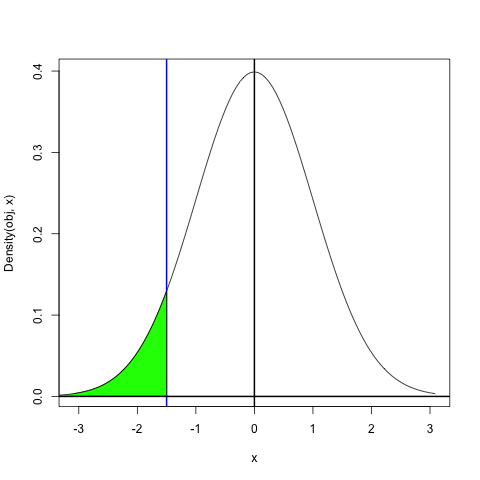
\includegraphics[width=5cm,height=4cm]{img/cours6Fig1}& \visible<3->{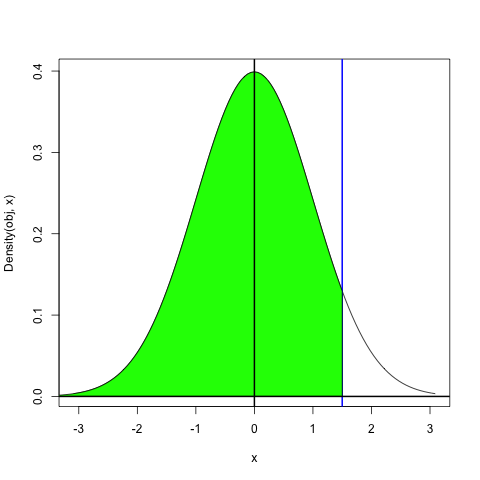
\includegraphics[width=5cm,height=4cm]{img/cours6Fig2}}
\end{tabular}
\begin{tikzpicture}[remember picture,overlay]
  \node [rotate=30,scale=10,text opacity=0.05]
    at (current page.center) {CQLS};
\end{tikzpicture}\end{frame}



\begin{frame}
\frametitle{}

{\small
\begin{block}{Choix du paramètre $d_\mu$ pour assertion d'intérêt $\mathbf{H_1}$: $\mu^{P1} > \mu^{P2}+20$ ?}
\begin{itemize}
\item Indications~\texttt{R}:\\
\texttt{\scriptsize> c(length(yP1),length(yP2),mean(yP1),mean(yP2))\\
$[1]$ 20 20 97.8735 74.879 \\
> pt(deltaEst.H0,length(yP1)+length(yP2)-2)\\
$[1]$ 0.8629092  \# p-valeur gauche}\pause
\item Deux choix possibles pour le paramètre $d_\mu$ et l'assertion d'intérêt~$\mathbf{H}_1$~:\\
{\scriptsize \begin{tabular}{|c|c|c|}\hline
paramètre & $d_\mu\!:=\!\mu^{P1} \!-\! \mu^{P2}$ & $d_\mu:=\mu^{P2} \!-\! \mu^{P1}$\\\hline
$\mathbf{H_1}$ & $d_\mu\!:=\!\mu^{P1} \!-\! \mu^{P2}\!>\!20$ & $\!d_\mu:=\mu^{P2} \!-\! \mu^{P1}\!<\!-20$ \\\hline
$\mathtt{deltaEst.H0}$ & $\Est{\delta_{d_\mu,20}}{y^{P1},y^{P2}}$ & $\Est{\delta_{d_\mu,-20}}{y^{P2},y^{P1}}$ \\\hline
$\mathtt{deltaEst.H0}$ & $\Est{d_\mu}{y^{P1},y^{P2}}\!-\!20\!$ & $\Est{d_\mu}{y^{P2},y^{P1}}\!-(-\!20\!)$\\
du signe de & $=\Est{\mu^{P1}}{y^{P1}}\!-\!\Est{\mu^{P2}}{y^{P2}}\!-\!20\!$ & $=\Est{\mu^{P2}}{y^{P2}}\!-\!\Est{\mu^{P1}}{y^{P1}}\!-(-\!20\!)$ \\\hline
\end{tabular}}\pause
\item {\scriptsize $\mathtt{deltaEst.H0}$ et $\Est{d_\mu}{y^{P1},y^{P2}}\!-\!20\!$ $\left\{\begin{array}{ccl} 
\mbox{mêmes signes} & \Rightarrow & \mathbf{H_1}: d_\mu\!:=\!\mu^{P1} \!-\! \mu^{P2}\!>\!20\\
\mbox{signes opposés} &\Rightarrow &  \mathbf{H_1}: d_\mu\!:=\!\mu^{P2} \!-\! \mu^{P1}\!<\!-20
\end{array}\right.$
}\pause
\end{itemize}
\end{block}
}
{\small
\begin{block}{}
\textbf{Application Numérique}~: $\mathtt{deltaEst.H0}>0$ puisque $p$-valeur$>50\%$ \pause et 
$\Est{\mu^{P1}}{y^{P1}}\!-\!\Est{\mu^{P2}}{y^{P2}}\!-\!20\!\NotR\! \texttt{mean(yP1)-mean(yP2)-20}\!\simeq\! 2.9945>0$.\\\pause
Mêmes signes $\Rightarrow$  \fbox{$\mathbf{H_1}$: $d_\mu\!:=\!\mu^{P1} \!-\! \mu^{P2}\!>\!20$}
\end{block}}
\begin{tikzpicture}[remember picture,overlay]
  \node [rotate=30,scale=10,text opacity=0.05]
    at (current page.center) {CQLS};
\end{tikzpicture}\end{frame}
 
\section{Rédaction des exemples}
\pgfdeclareimage[width=8cm,height=4cm,interpolate=true]{pvalcaq1}{img/pvalcaq1}


\pgfdeclareimage[width=8cm,height=4cm,interpolate=true]{pvalcaq1b}{img/pvalcaq1b}

\pgfdeclareimage[width=8cm,height=4cm,interpolate=true]{pvalcaq2}{img/pvalcaq2}

\pgfdeclareimage[width=8cm,height=4cm,interpolate=true]{pvalcaq3a}{img/pvalcaq3a}

\pgfdeclareimage[width=8cm,height=4cm,interpolate=true]{pvalcaq3b}{img/pvalcaq3b}


\pgfdeclareimage[width=8cm,height=4cm,interpolate=true]{pvalcaq4a}{img/pvalcaq4a}

\pgfdeclareimage[width=8cm,height=4cm,interpolate=true]{pvalcaq4b}{img/pvalcaq4b}

\pgfdeclareimage[width=8cm,height=4cm,interpolate=true]{pvalcaq5a}{img/pvalcaq5a}

\pgfdeclareimage[width=8cm,height=4cm,interpolate=true]{pvalcaq5b}{img/pvalcaq5b}


%\beamertemplateshadingbackground{green!50}{yellow!50}
\begin{frame}<1->
\setbeamercolor{header}{fg=black,bg=blue!40!white}
 \hspace*{2.5cm}\begin{beamerboxesrounded}[width=6cm,shadow=true,lower=header]{}
  \pgfsetxvec{\pgfpoint{6cm}{0cm}}
\pgfsetyvec{\pgfpoint{0cm}{0.5cm}}
\begin{pgfpicture}{0cm}{0cm}{6cm}{0.5cm}

  \only<1-11>{
\pgfputat{\pgfxy(0.5,0.5)}{\pgfbox[center,center]{\textbf{\large Chiffre Affaires - Question 1a}}}}
\only<12-22>{
\pgfputat{\pgfxy(0.5,0.5)}{\pgfbox[center,center]{\textbf{\large Chiffre Affaires - Question 1b}}}}
\only<23-33>{
\pgfputat{\pgfxy(0.5,0.5)}{\pgfbox[center,center]{\textbf{\large Chiffre Affaires - Question 2}}}}
\only<34-44>{
\pgfputat{\pgfxy(0.5,0.5)}{\pgfbox[center,center]{\textbf{\large Chiffre Affaires - Question 3a}}}}
\only<45-55>{
\pgfputat{\pgfxy(0.5,0.5)}{\pgfbox[center,center]{\textbf{\large Chiffre Affaires - Question 3b}}}}
\only<56-66>{
\pgfputat{\pgfxy(0.5,0.5)}{\pgfbox[center,center]{\textbf{\large Chiffre Affaires - Question 4a}}}}
\only<67-77>{
\pgfputat{\pgfxy(0.5,0.5)}{\pgfbox[center,center]{\textbf{\large Chiffre Affaires - Question 4b}}}}
\only<78-88>{
\pgfputat{\pgfxy(0.5,0.5)}{\pgfbox[center,center]{\textbf{\large Chiffre Affaires - Question 5a}}}}
\only<89-99>{
\pgfputat{\pgfxy(0.5,0.5)}{\pgfbox[center,center]{\textbf{\large Chiffre Affaires - Question 5b}}}}

  \end{pgfpicture}

\end{beamerboxesrounded}

\setbeamercolor{postit}{fg=black,bg=green!40!white}
%\begin{beamercolorbox}[sep=1em,wd=12cm]{postit}
\begin{beamerboxesrounded}[shadow=true,lower=postit]{}
\pgfsetxvec{\pgfpoint{11cm}{0cm}}
\pgfsetyvec{\pgfpoint{0cm}{2.1cm}}
\begin{pgfpicture}{0cm}{0cm}{11cm}{2.1cm}

\only<1-2>{
\pgfputat{\pgfxy(0.5,1.0)}{\pgfbox[center,top]{\begin{minipage}{11cm}\textbf{Question } Comment s'écrit l'assertion d'intérêt $\mathbf{H_1}$ en fonction des paramètres d'intérêt et d'écart~?\only<1>{\\\textbf{Assertion d'intérêt}~: le chiffre d'affaires annuel moyen des PME du pays P1 est de plus de 20 unités supérieur à celui du pays P2}\only<2>{\\ \centerline{$\mathbf{H_1}$:$d_\mu:=\mu^{P1}-\mu^{P2}>20$ $\Longleftrightarrow$ $\delta_{d_\mu,20}:={\displaystyle \frac{d_\mu-20}{
\sigma_{\cqlshat{d_\mu}}
}} >0$}}
\end{minipage}}}}
\only<3-4>{
\pgfputat{\pgfxy(0.5,1.0)}{\pgfbox[center,top]{\begin{minipage}{11cm}\textbf{Question }: Quelle est la pire des situations, i.e. parmi toutes les situations quelle est celle qui engendre le plus grand risque d'erreur de première espèce~?\end{minipage}}}}
\only<5-6>{
\pgfputat{\pgfxy(0.5,1.0)}{\pgfbox[center,top]{\begin{minipage}{11cm}\textbf{Question }: Quelle est l'information du mathématicien quant au comportement de $\Est{\delta_{d_\mu,20}}{Y^{P1},Y^{P2}}$ dans la pire des situations~?\end{minipage}}}}
\only<7-8>{
\pgfputat{\pgfxy(0.5,1.0)}{\pgfbox[center,top]{\begin{minipage}{11cm}\textbf{Question }: Comment s'écrit la règle de décision ne produisant pas plus de 5\% d'erreur de première espèce~? \\
\textbf{Indic \texttt{R}}~: \texttt{deltaEst.H0}$\simeq$\texttt{1.109512}\\\phantom{\textbf{Indic \texttt{R}}~: }\texttt{qt(0.95,38)}$\simeq$ \texttt{1.685954}
\end{minipage}}}}
\only<9-11>{
\pgfputat{\pgfxy(0.5,1.0)}{\pgfbox[center,top]{\begin{minipage}{11cm}\textbf{Question }: Comment conclueriez-vous au vu des données \texttt{yP1} et \texttt{yP2} en \texttt{R}~?\\
\textbf{Indic \texttt{R}}~: \texttt{deltaEst.H0}$\simeq$\texttt{1.109512}\\\phantom{\textbf{Indic \texttt{R}}~: }\texttt{qt(0.95,38)}$\simeq$ \texttt{1.685954} 
\end{minipage}}}}
\only<12-13>{
\pgfputat{\pgfxy(0.5,1.0)}{\pgfbox[center,top]{\begin{minipage}{11cm}\textbf{Question } Comment s'écrit l'assertion d'intérêt $\mathbf{H_1}$ en fonction des paramètres d'intérêt et d'écart~?\only<12>{\\\textbf{Assertion d'intérêt}~: le chiffre d'affaires annuel moyen des PME du pays P1 est de plus de 20 unités supérieur à celui du pays P2}\only<13>{\\ \centerline{$\mathbf{H_1}$:$d_\mu:=\mu^{P1}-\mu^{P2}>20$ $\Longleftrightarrow$ $\delta_{d_\mu,20}:={\displaystyle \frac{d_\mu-20}{
\sigma_{\cqlshat{d_\mu}}
}} >0$}}
\end{minipage}}}}
\only<14-15>{
\pgfputat{\pgfxy(0.5,1.0)}{\pgfbox[center,top]{\begin{minipage}{11cm}\textbf{Question }: Quelle est la pire des situations, i.e. parmi toutes les situations quelle est celle qui engendre le plus grand risque d'erreur de première espèce~?\end{minipage}}}}
\only<16-17>{
\pgfputat{\pgfxy(0.5,1.0)}{\pgfbox[center,top]{\begin{minipage}{11cm}\textbf{Question }: Quelle est l'information du mathématicien quant au comportement de $\Est{\delta_{d_\mu,20}}{Y^{P1},Y^{P2}}$ dans la pire des situations~?\end{minipage}}}}
\only<18-19>{
\pgfputat{\pgfxy(0.5,1.0)}{\pgfbox[center,top]{\begin{minipage}{11cm}\textbf{Question }: Comment s'écrit la règle de décision ne produisant pas plus de 5\% d'erreur de première espèce~? \\
\textbf{Indic \texttt{R}}~: \texttt{pnorm(deltaEst.H0)}$\simeq$ \texttt{0.9825057}\end{minipage}}}}
\only<20-22>{
\pgfputat{\pgfxy(0.5,1.0)}{\pgfbox[center,top]{\begin{minipage}{11cm}\textbf{Question }: Comment conclueriez-vous au vu des données \texttt{yP1} et \texttt{yP2} en \texttt{R}~?\\
\textbf{Indic \texttt{R}}~: \texttt{pnorm(deltaEst.H0)}$\simeq$ \texttt{0.9825057}\end{minipage}}}}
\only<23-24>{
\pgfputat{\pgfxy(0.5,1.0)}{\pgfbox[center,top]{\begin{minipage}{11cm}\textbf{Question } Comment s'écrit l'assertion d'intérêt $\mathbf{H_1}$ en fonction des paramètres d'intérêt et d'écart~?\only<23>{\\\textbf{Assertion d'intérêt}~: le C.A. annuel moyen des PME du pays P1 est de plus de 20\% supérieur à celui du pays P2}\only<24>{\\ \centerline{$\mathbf{H_1}$:$r_\mu:=\displaystyle \frac{\mu^{P1}}{\mu^{P2}}>1.2$ $\Longleftrightarrow$ $\delta_{r_\mu,1.2}:={\displaystyle \frac{r_\mu-1.2}{
\sigma_{\cqlshat{r_\mu}}
}} >0$}}
\end{minipage}}}}
\only<25-26>{
\pgfputat{\pgfxy(0.5,1.0)}{\pgfbox[center,top]{\begin{minipage}{11cm}\textbf{Question }: Quelle est la pire des situations, i.e. parmi toutes les situations quelle est celle qui engendre le plus grand risque d'erreur de première espèce~?\end{minipage}}}}
\only<27-28>{
\pgfputat{\pgfxy(0.5,1.0)}{\pgfbox[center,top]{\begin{minipage}{11cm}\textbf{Question }: Quelle est l'information du mathématicien quant au comportement de $\Est{\delta_{r_\mu,1.2}}{Y^{P1},Y^{P2}}$ dans la pire des situations~?\end{minipage}}}}
\only<29-30>{
\pgfputat{\pgfxy(0.5,1.0)}{\pgfbox[center,top]{\begin{minipage}{11cm}\textbf{Question }: Comment s'écrit la règle de décision ne produisant pas plus de 5\% d'erreur de première espèce~? \\
\textbf{Indic \texttt{R}}~: \texttt{deltaEst.H0}$\simeq$\texttt{4.155933}\\\phantom{\textbf{Indic \texttt{R}}~: }\texttt{qnorm(0.95)}$\simeq$ \texttt{1.644854}
\end{minipage}}}}
\only<31-33>{
\pgfputat{\pgfxy(0.5,1.0)}{\pgfbox[center,top]{\begin{minipage}{11cm}\textbf{Question }: Comment conclueriez-vous au vu des données \texttt{yP1} et \texttt{yP2} en \texttt{R}~?\\
\textbf{Indic \texttt{R}}~: \texttt{deltaEst.H0}$\simeq$\texttt{4.155933}\\\phantom{\textbf{Indic \texttt{R}}~: }\texttt{qnorm(0.95)}$\simeq$ \texttt{1.644854} 
\end{minipage}}}}
\only<34-35>{
\pgfputat{\pgfxy(0.5,1.0)}{\pgfbox[center,top]{\begin{minipage}{11cm}\textbf{Question } Comment s'écrit l'assertion d'intérêt $\mathbf{H_1}$ en fonction des paramètres d'intérêt et d'écart~?\only<34>{\\\textbf{Assertion d'intérêt}~: les hétérogénéités des chiffres d'affaires annuels des PME des deux pays diffèrent}\only<35>{\\ \centerline{$\mathbf{H_1}$:$r_{\sigma^2}:=\displaystyle \frac{\sigma^2_{P1}}{\sigma^2_{P2}}\neq1$ $\Longleftrightarrow$ $\delta_{r_{\sigma^2},1}:={\displaystyle \frac{r_{\sigma^2}}{1}}\neq1$}}
\end{minipage}}}}
\only<36-37>{
\pgfputat{\pgfxy(0.5,1.0)}{\pgfbox[center,top]{\begin{minipage}{11cm}\textbf{Question }: Quelle est la pire des situations, i.e. parmi toutes les situations quelle est celle qui engendre le plus grand risque d'erreur de première espèce~?\end{minipage}}}}
\only<38-39>{
\pgfputat{\pgfxy(0.5,1.0)}{\pgfbox[center,top]{\begin{minipage}{11cm}\textbf{Question }: Quelle est l'information du mathématicien quant au comportement de $\Est{\delta_{r_{\sigma^2},1}}{Y^{P1},Y^{P2}}$ dans la pire des situations~?\end{minipage}}}}
\only<40-41>{
\pgfputat{\pgfxy(0.5,1.0)}{\pgfbox[center,top]{\begin{minipage}{11cm}\textbf{Question }: Comment s'écrit la règle de décision ne produisant pas plus de 5\% d'erreur de première espèce~? \\
\textbf{Indic \texttt{R}}~: \texttt{pf(deltaEst.H0,19,19)}$\simeq$ \texttt{0.9609953}\end{minipage}}}}
\only<42-44>{
\pgfputat{\pgfxy(0.5,1.0)}{\pgfbox[center,top]{\begin{minipage}{11cm}\textbf{Question }: Comment conclueriez-vous au vu des données \texttt{yP1} et \texttt{yP2} en \texttt{R}~?\\
\textbf{Indic \texttt{R}}~: \texttt{pf(deltaEst.H0,19,19)}$\simeq$ \texttt{0.9609953}\end{minipage}}}}
\only<45-46>{
\pgfputat{\pgfxy(0.5,1.0)}{\pgfbox[center,top]{\begin{minipage}{11cm}\textbf{Question } Comment s'écrit l'assertion d'intérêt $\mathbf{H_1}$ en fonction des paramètres d'intérêt et d'écart~?\only<45>{\\\textbf{Assertion d'intérêt}~: les hétérogénéités des chiffres d'affaires annuels des PME des deux pays diffèrent}\only<46>{\\ \centerline{$\mathbf{H_1}$:$d_{\sigma^2}:=\sigma^2_{P1}-\sigma^2_{P2}\neq0$ $\Longleftrightarrow$ $\delta_{d_{\sigma^2},0}:={\displaystyle \frac{d_{\sigma^2}-0}{
\sigma_{\cqlshat{d_{\sigma^2}}}
}} \neq0$}}
\end{minipage}}}}
\only<47-48>{
\pgfputat{\pgfxy(0.5,1.0)}{\pgfbox[center,top]{\begin{minipage}{11cm}\textbf{Question }: Quelle est la pire des situations, i.e. parmi toutes les situations quelle est celle qui engendre le plus grand risque d'erreur de première espèce~?\end{minipage}}}}
\only<49-50>{
\pgfputat{\pgfxy(0.5,1.0)}{\pgfbox[center,top]{\begin{minipage}{11cm}\textbf{Question }: Quelle est l'information du mathématicien quant au comportement de $\Est{\delta_{d_{\sigma^2},0}}{Y^{P1},Y^{P2}}$ dans la pire des situations~?\end{minipage}}}}
\only<51-52>{
\pgfputat{\pgfxy(0.5,1.0)}{\pgfbox[center,top]{\begin{minipage}{11cm}\textbf{Question }: Comment s'écrit la règle de décision ne produisant pas plus de 5\% d'erreur de première espèce~? \\
\textbf{Indic \texttt{R}}~: \texttt{pnorm(deltaEst.H0)}$\simeq$ \texttt{0.9748944}\end{minipage}}}}
\only<53-55>{
\pgfputat{\pgfxy(0.5,1.0)}{\pgfbox[center,top]{\begin{minipage}{11cm}\textbf{Question }: Comment conclueriez-vous au vu des données \texttt{yP1} et \texttt{yP2} en \texttt{R}~?\\
\textbf{Indic \texttt{R}}~: \texttt{pnorm(deltaEst.H0)}$\simeq$ \texttt{0.9748944}\end{minipage}}}}
\only<56-57>{
\pgfputat{\pgfxy(0.5,1.0)}{\pgfbox[center,top]{\begin{minipage}{11cm}\textbf{Question } Comment s'écrit l'assertion d'intérêt $\mathbf{H_1}$ en fonction des paramètres d'intérêt et d'écart~?\only<56>{\\\textbf{Assertion d'intérêt}~: l'hétérogénéité des C.A. annuels des PME de P1 est de plus de 25\% supérieure à celle de P2}\only<57>{\\ \centerline{$\mathbf{H_1}$:$r_{\sigma^2}:=\displaystyle \frac{\sigma^2_{P1}}{\sigma^2_{P2}}>1.25$ $\Longleftrightarrow$ $\delta_{r_{\sigma^2},1.25}:={\displaystyle \frac{r_{\sigma^2}}{1.25}}>1$}}
\end{minipage}}}}
\only<58-59>{
\pgfputat{\pgfxy(0.5,1.0)}{\pgfbox[center,top]{\begin{minipage}{11cm}\textbf{Question }: Quelle est la pire des situations, i.e. parmi toutes les situations quelle est celle qui engendre le plus grand risque d'erreur de première espèce~?\end{minipage}}}}
\only<60-61>{
\pgfputat{\pgfxy(0.5,1.0)}{\pgfbox[center,top]{\begin{minipage}{11cm}\textbf{Question }: Quelle est l'information du mathématicien quant au comportement de $\Est{\delta_{r_{\sigma^2},1.25}}{Y^{P1},Y^{P2}}$ dans la pire des situations~?\end{minipage}}}}
\only<62-63>{
\pgfputat{\pgfxy(0.5,1.0)}{\pgfbox[center,top]{\begin{minipage}{11cm}\textbf{Question }: Comment s'écrit la règle de décision ne produisant pas plus de 5\% d'erreur de première espèce~? \\
\textbf{Indic \texttt{R}}~: \texttt{pf(deltaEst.H0,19,19)}$\simeq$ \texttt{0.9026961}\end{minipage}}}}
\only<64-66>{
\pgfputat{\pgfxy(0.5,1.0)}{\pgfbox[center,top]{\begin{minipage}{11cm}\textbf{Question }: Comment conclueriez-vous au vu des données \texttt{yP1} et \texttt{yP2} en \texttt{R}~?\\
\textbf{Indic \texttt{R}}~: \texttt{pf(deltaEst.H0,19,19)}$\simeq$ \texttt{0.9026961}\end{minipage}}}}
\only<67-68>{
\pgfputat{\pgfxy(0.5,1.0)}{\pgfbox[center,top]{\begin{minipage}{11cm}\textbf{Question } Comment s'écrit l'assertion d'intérêt $\mathbf{H_1}$ en fonction des paramètres d'intérêt et d'écart~?\only<67>{\\\textbf{Assertion d'intérêt}~: l'hétérogénéité des C.A. annuels des PME de P1 est de plus de 25\% supérieure à celle de P2}\only<68>{\\ \centerline{$\mathbf{H_1}$:$r_{\sigma^2}:=\displaystyle \frac{\sigma^2_{P1}}{\sigma^2_{P2}}>1.25$ $\Longleftrightarrow$ $\delta_{r_{\sigma^2},1.25}:={\displaystyle \frac{r_{\sigma^2}-1.25}{
\sigma_{\cqlshat{r_{\sigma^2}}}
}} >0$}}
\end{minipage}}}}
\only<69-70>{
\pgfputat{\pgfxy(0.5,1.0)}{\pgfbox[center,top]{\begin{minipage}{11cm}\textbf{Question }: Quelle est la pire des situations, i.e. parmi toutes les situations quelle est celle qui engendre le plus grand risque d'erreur de première espèce~?\end{minipage}}}}
\only<71-72>{
\pgfputat{\pgfxy(0.5,1.0)}{\pgfbox[center,top]{\begin{minipage}{11cm}\textbf{Question }: Quelle est l'information du mathématicien quant au comportement de $\Est{\delta_{r_{\sigma^2},1.25}}{Y^{P1},Y^{P2}}$ dans la pire des situations~?\end{minipage}}}}
\only<73-74>{
\pgfputat{\pgfxy(0.5,1.0)}{\pgfbox[center,top]{\begin{minipage}{11cm}\textbf{Question }: Comment s'écrit la règle de décision ne produisant pas plus de 5\% d'erreur de première espèce~? \\
\textbf{Indic \texttt{R}}~: \texttt{pnorm(deltaEst.H0)}$\simeq$ \texttt{0.8334422}\end{minipage}}}}
\only<75-77>{
\pgfputat{\pgfxy(0.5,1.0)}{\pgfbox[center,top]{\begin{minipage}{11cm}\textbf{Question }: Comment conclueriez-vous au vu des données \texttt{yP1} et \texttt{yP2} en \texttt{R}~?\\
\textbf{Indic \texttt{R}}~: \texttt{pnorm(deltaEst.H0)}$\simeq$ \texttt{0.8334422}\end{minipage}}}}
\only<78-79>{
\pgfputat{\pgfxy(0.5,1.0)}{\pgfbox[center,top]{\begin{minipage}{11cm}\textbf{Question } Comment s'écrit l'assertion d'intérêt $\mathbf{H_1}$ en fonction des paramètres d'intérêt et d'écart~?\only<78>{\\\textbf{Assertion d'intérêt}~: le chiffre d'affaires annuel moyen des PME a augmenté entre 2004 et 2005 de 10 unités}\only<79>{\\ \centerline{$\mathbf{H_1}$:$\mu^{D}<-10$ $\Longleftrightarrow$ $\delta_{\mu^{D},-10}:={\displaystyle \frac{\mu^{D}-(-10)}{
\sigma_{\cqlshat{\mu^{D}}}
}} <0$}}
\end{minipage}}}}
\only<80-81>{
\pgfputat{\pgfxy(0.5,1.0)}{\pgfbox[center,top]{\begin{minipage}{11cm}\textbf{Question }: Quelle est la pire des situations, i.e. parmi toutes les situations quelle est celle qui engendre le plus grand risque d'erreur de première espèce~?\end{minipage}}}}
\only<82-83>{
\pgfputat{\pgfxy(0.5,1.0)}{\pgfbox[center,top]{\begin{minipage}{11cm}\textbf{Question }: Quelle est l'information du mathématicien quant au comportement de $\Est{\delta_{\mu^{D},-10}}{Y^{D}}$ dans la pire des situations~?\end{minipage}}}}
\only<84-85>{
\pgfputat{\pgfxy(0.5,1.0)}{\pgfbox[center,top]{\begin{minipage}{11cm}\textbf{Question }: Comment s'écrit la règle de décision ne produisant pas plus de 5\% d'erreur de première espèce~? \\
\textbf{Indic \texttt{R}}~: \texttt{pt(deltaEst.H0,19)}$\simeq$ \texttt{0.06435257}\end{minipage}}}}
\only<86-88>{
\pgfputat{\pgfxy(0.5,1.0)}{\pgfbox[center,top]{\begin{minipage}{11cm}\textbf{Question }: Comment conclueriez-vous au vu des données \texttt{y04-y05} en \texttt{R}~?\\
\textbf{Indic \texttt{R}}~: \texttt{pt(deltaEst.H0,19)}$\simeq$ \texttt{0.06435257}\end{minipage}}}}
\only<89-90>{
\pgfputat{\pgfxy(0.5,1.0)}{\pgfbox[center,top]{\begin{minipage}{11cm}\textbf{Question } Comment s'écrit l'assertion d'intérêt $\mathbf{H_1}$ en fonction des paramètres d'intérêt et d'écart~?\only<89>{\\\textbf{Assertion d'intérêt}~: le chiffre d'affaires annuel moyen des PME a augmenté entre 2004 et 2005 de 10 unités}\only<90>{\\ \centerline{$\mathbf{H_1}$:$\mu^{D}<-10$ $\Longleftrightarrow$ $\delta_{\mu^{D},-10}:={\displaystyle \frac{\mu^{D}-(-10)}{
\sigma_{\cqlshat{\mu^{D}}}
}} <0$}}
\end{minipage}}}}
\only<91-92>{
\pgfputat{\pgfxy(0.5,1.0)}{\pgfbox[center,top]{\begin{minipage}{11cm}\textbf{Question }: Quelle est la pire des situations, i.e. parmi toutes les situations quelle est celle qui engendre le plus grand risque d'erreur de première espèce~?\end{minipage}}}}
\only<93-94>{
\pgfputat{\pgfxy(0.5,1.0)}{\pgfbox[center,top]{\begin{minipage}{11cm}\textbf{Question }: Quelle est l'information du mathématicien quant au comportement de $\Est{\delta_{\mu^{D},-10}}{Y^{D}}$ dans la pire des situations~?\end{minipage}}}}
\only<95-96>{
\pgfputat{\pgfxy(0.5,1.0)}{\pgfbox[center,top]{\begin{minipage}{11cm}\textbf{Question }: Comment s'écrit la règle de décision ne produisant pas plus de 5\% d'erreur de première espèce~? \\
\textbf{Indic \texttt{R}}~: \texttt{pnorm(deltaEst.H0)}$\simeq$ \texttt{0.01285186}\end{minipage}}}}
\only<97-99>{
\pgfputat{\pgfxy(0.5,1.0)}{\pgfbox[center,top]{\begin{minipage}{11cm}\textbf{Question }: Comment conclueriez-vous au vu des données \texttt{y04-y05} en \texttt{R}~?\\
\textbf{Indic \texttt{R}}~: \texttt{pnorm(deltaEst.H0)}$\simeq$ \texttt{0.01285186}\end{minipage}}}}

\end{pgfpicture}

\end{beamerboxesrounded}
%\end{beamercolorbox}

\setbeamercolor{postex}{fg=black,bg=yellow!50!white}
%\begin{beamercolorbox}[sep=1em,wd=12cm]{postex}
\begin{beamerboxesrounded}[shadow=true,lower=postex]{}
\pgfsetxvec{\pgfpoint{11cm}{0cm}}
\pgfsetyvec{\pgfpoint{0cm}{5cm}}
\begin{pgfpicture}{0cm}{0cm}{11cm}{5cm}

\only<1-11>{
\pgfputat{\pgfxy(0.5,1.0)}{\pgfbox[center,top]{\begin{minipage}{11cm}\only<1>{\textbf{Indications \texttt{R}}~:\\\texttt{  > c(length(yP1),length(yP2))\\
$[1]$ 20 20\\
> mean(yP1)\\
$[1]$ 97.8735\\
> mean(yP2)\\
$[1]$ 74.879\\
  > deltaEst.H0 \# instruction R à fournir\\
$[1]$ 1.109512\\
> qt(0.95,38)\\
$[1]$ 1.685954}}\visible<2-11>{\noindent\textbf{Hypothèses de test~:}}\visible<4-11>{ {\small $\mathbf{H}_0:$ $d_\mu=20$} vs } \visible<2-11>{$\mathbf{H}_1:$ $d_\mu>20$}\\\only<2>{\\\noindent \textbf{Préliminaire} : puisque $\mathtt{(mean(yP1)-mean(yP2)-20)}\simeq2.9945$ est du même signe (i.e. positif) que $\mathtt{deltaEst.H0}$ , on a~: 
      \begin{itemize}
\item \textit{paramètre d'intérêt}~: $d_\mu=\mu^{P1}-\mu^{P2}$
\item \textit{sa future estimation}~: $\Est{d_\mu}{Y^{P1},Y^{P2}}=\Est{\mu^{P1}}{Y^{P1}}-\Est{\mu^{P2}}{Y^{P2}}$
\end{itemize}}\visible<6-11>{\noindent\textbf{Statistique de test sous $\mathbf{H_0}$~:}\\
\centerline{$\Est{\delta_{d_\mu,20}}{Y^{P1},Y^{P2}}= {\displaystyle \frac{\Est{d_\mu}{Y^{P1},Y^{P2}}-20}{
\Est{\sigma_{\cqlshat{d_\mu}}}{Y^{P1},Y^{P2}}
}} 
  \leadsto\mathcal{S}t(20+20-2)  $}\newline}
\visible<8-11>{\noindent\textbf{Règle de Décision}~:\\
\centerline{Accepter $\mathbf{H_1}$ si   ${\color<10>{orange}\Est{\delta_{d_\mu,20}}{y^{P1},y^{P2}}} > {\color<10>{darkgreen}\delta^+_{lim,5\%}}$}\newline}
\visible<10-11>{\small\noindent\textbf{Conclusion}~: puisqu'au vu des données,
\\$\Est{\delta_{d_\mu,20}}{y^{P1},y^{P2}}\!\NotR\! {\color<10>{orange}\mbox{\scriptsize\texttt{(mean(yP1)-mean(yP2)-20)/seDMeanG(yP1,yP2)}}\!\simeq\! 1.11}$\\\phantom{$\!\Est{\delta_{d_\mu,20}}{y^{P1},y^{P2}}\!$}$\!\ngtr \delta^+_{lim,5\%}\!
\NotR\!{\color<10>{darkgreen}\mathtt{qt(1-.05,38)\!\simeq\!1.686}}\!$\\
 on ne peut pas plutôt penser (avec un risque de 5\%) que le chiffre d'affaires annuel moyen des PME du pays P1 est de plus de 20 unités supérieur à celui du pays P2.}\end{minipage}}}}
\only<10>{
\pgfputat{\pgfxy(0.15,0.65)}{\pgfbox[left,bottom]{\pgfuseimage{pvalcaq1}}}}
\only<12-22>{
\pgfputat{\pgfxy(0.5,1.0)}{\pgfbox[center,top]{\begin{minipage}{11cm}\only<12>{\textbf{Indications \texttt{R}}~:\\\texttt{  > c(length(yP1),length(yP2))\\
$[1]$ 40 40\\
> mean(yP1)\\
$[1]$ 99.50575\\
> mean(yP2)\\
$[1]$ 75.467\\
  > pnorm(deltaEst.H0)\\
$[1]$ 0.9825057}}\visible<13-22>{\noindent\textbf{Hypothèses de test~:}}\visible<15-22>{ {\small $\mathbf{H}_0:$ $d_\mu=20$} vs } \visible<13-22>{$\mathbf{H}_1:$ $d_\mu>20$}\\\only<13>{\\\noindent \textbf{Préliminaire} : puisque $\mathtt{(mean(yP1)-mean(yP2)-20)}\simeq4.03875$ est du même signe (i.e. positif) que $\mathtt{deltaEst.H0}$ (car p-valeur gauche supérieure à $50\%$), on a~: 
      \begin{itemize}
\item \textit{paramètre d'intérêt}~: $d_\mu=\mu^{P1}-\mu^{P2}$
\item \textit{sa future estimation}~: $\Est{d_\mu}{Y^{P1},Y^{P2}}=\Est{\mu^{P1}}{Y^{P1}}-\Est{\mu^{P2}}{Y^{P2}}$
\end{itemize}}\visible<17-22>{\noindent\textbf{Statistique de test sous $\mathbf{H_0}$~:}\\
\centerline{$\Est{\delta_{d_\mu,20}}{Y^{P1},Y^{P2}}= {\displaystyle \frac{\Est{d_\mu}{Y^{P1},Y^{P2}}-20}{
\Est{\sigma_{\cqlshat{d_\mu}}}{Y^{P1},Y^{P2}}
}} 
  \SuitApprox\mathcal{N}(0,1) $}\newline}
\visible<19-22>{\noindent\textbf{Règle de Décision}~:\\
\centerline{Accepter $\mathbf{H_1}$ si   {\color<21>{orange}p-valeur (droite)} < {\color<21>{blue}5\%}}\newline}
\visible<21-22>{\small\noindent\textbf{Conclusion}~: puisqu'au vu des données,
\\ \texttt{p-valeur}$\NotR{\color<21>{orange}\mathtt{1-pnorm((mean(yP1)-mean(yP2)-20)/seDMean(yP1,yP2))}}$\\ \phantom{\texttt{p-valeur}}${\color<21>{orange}\simeq 1.75\%}<{\color<21>{blue}5\%}$\\
 on peut plutôt penser (avec un risque de 5\%) que le chiffre d'affaires annuel moyen des PME du pays P1 est de plus de 20 unités supérieur à celui du pays P2.}\end{minipage}}}}
\only<21>{
\pgfputat{\pgfxy(0.15,0.65)}{\pgfbox[left,bottom]{\pgfuseimage{pvalcaq1b}}}}
\only<23-33>{
\pgfputat{\pgfxy(0.5,1.0)}{\pgfbox[center,top]{\begin{minipage}{11cm}\only<23>{\textbf{Indications \texttt{R}}~:\\\texttt{  > c(length(yP1),length(yP2))\\
$[1]$ 40 40\\
> mean(yP1)\\
$[1]$ 99.50575\\
> mean(yP2)\\
$[1]$ 75.467\\
  > deltaEst.H0 \# instruction R à fournir\\
$[1]$ 4.155933\\
> qnorm(0.95)\\
$[1]$ 1.644854}}\visible<24-33>{\noindent\textbf{Hypothèses de test~:}}\visible<26-33>{ {\small $\mathbf{H}_0:$ $r_\mu=1.2$} vs } \visible<24-33>{$\mathbf{H}_1:$ $r_\mu>1.2$}\\\only<24>{\\\noindent \textbf{Préliminaire} : puisque $\mathtt{(mean(yP1)/mean(yP2)-1.2)}\simeq0.1185333$ est du même signe (i.e. positif) que $\mathtt{deltaEst.H0}$ , on a~: 
      \begin{itemize}
\item \textit{paramètre d'intérêt}~: $r_\mu=\displaystyle \frac{\mu^{P1}}{\mu^{P2}}$
\item \textit{sa future estimation}~: $\Est{r_\mu}{Y^{P1},Y^{P2}}=\Est{\mu^{P1}}{Y^{P1}}/\Est{\mu^{P2}}{Y^{P2}}$
\end{itemize}}\visible<28-33>{\noindent\textbf{Statistique de test sous $\mathbf{H_0}$~:}\\
\centerline{$\Est{\delta_{r_\mu,1.2}}{Y^{P1},Y^{P2}}= {\displaystyle \frac{\Est{r_\mu}{Y^{P1},Y^{P2}}-1.2}{
\Est{\sigma_{\cqlshat{r_\mu}}}{Y^{P1},Y^{P2}}
}} 
  \SuitApprox\mathcal{N}(0,1) $}\newline}
\visible<30-33>{\noindent\textbf{Règle de Décision}~:\\
\centerline{Accepter $\mathbf{H_1}$ si   ${\color<32>{orange}\Est{\delta_{r_\mu,1.2}}{y^{P1},y^{P2}}} > {\color<32>{darkgreen}\delta^+_{lim,5\%}}$}\newline}
\visible<32-33>{\small\noindent\textbf{Conclusion}~: puisqu'au vu des données,
\\$\Est{\delta_{r_\mu,1.2}}{y^{P1},y^{P2}}\!\NotR\! {\color<32>{orange}\mbox{\scriptsize\texttt{(mean(yP1)/mean(yP2)-1.2)/seRMean(yP1,yP2)}}\!\simeq\! 4.156}$\\\phantom{$\!\Est{\delta_{r_\mu,1.2}}{y^{P1},y^{P2}}\!$}$\!> \delta^+_{lim,5\%}\!
\NotR\!{\color<32>{darkgreen}\mathtt{qnorm(1-.05)\!\simeq\!1.645}}\!$\\
 on peut plutôt penser (avec un risque de 5\%) que le C.A. annuel moyen des PME du pays P1 est de plus de 20\% supérieur à celui du pays P2.}\end{minipage}}}}
\only<32>{
\pgfputat{\pgfxy(0.15,0.65)}{\pgfbox[left,bottom]{\pgfuseimage{pvalcaq2}}}}
\only<34-44>{
\pgfputat{\pgfxy(0.5,1.0)}{\pgfbox[center,top]{\begin{minipage}{11cm}\only<34>{\textbf{Indications \texttt{R}}~:\\\texttt{  > c(length(yP1),length(yP2))\\
$[1]$ 20 20\\
> var(yP1)\\
$[1]$ 101.4692\\
> var(yP2)\\
$[1]$ 44.21577\\
  > pf(deltaEst.H0,19,19)\\
$[1]$ 0.9609953}}\visible<35-44>{\noindent\textbf{Hypothèses de test~:}}\visible<37-44>{ {\small $\mathbf{H}_0:$ $r_{\sigma^2}=1$} vs } \visible<35-44>{$\mathbf{H}_1:$ $r_{\sigma^2}\neq1$}\\\only<35>{\\\noindent \textbf{Préliminaire} : \begin{itemize}
\item \textit{paramètre d'intérêt}~: $r_{\sigma^2}=\displaystyle \frac{\sigma^2_{P1}}{\sigma^2_{P2}}$
\item \textit{sa future estimation}~: $\Est{r_{\sigma^2}}{Y^{P1},Y^{P2}}=\Est{\sigma^2_{P1}}{Y^{P1}}/\Est{\sigma^2_{P2}}{Y^{P2}}$
\end{itemize}}\visible<39-44>{\noindent\textbf{Statistique de test sous $\mathbf{H_0}$~:}\\
\centerline{$\Est{\delta_{r_{\sigma^2},1}}{Y^{P1},Y^{P2}}= {\displaystyle \frac{\Est{r_{\sigma^2}}{Y^{P1},Y^{P2}}}{1}} 
  \leadsto\mathcal{F}(20-1,20-1)  $}\newline}
\visible<41-44>{\noindent\textbf{Règle de Décision}~:\\
\centerline{Accepter $\mathbf{H_1}$ si   {\color<43>{orange}p-valeur (biltatérale)} < {\color<43>{blue}5\%}}\newline}
\visible<43-44>{\small\noindent\textbf{Conclusion}~: puisqu'au vu des données,
\\ \texttt{p-valeur}$\NotR{\color<43>{orange}\mathtt{2*(1-pf((var(yP1)/var(yP2))/1,19,19))}}$\\ \phantom{\texttt{p-valeur}}${\color<43>{orange}\simeq 7.8\%}\nless{\color<43>{blue}5\%}$\\
 on ne peut pas plutôt penser (avec un risque de 5\%) que les hétérogénéités des chiffres d'affaires annuels des PME des deux pays diffèrent.}\end{minipage}}}}
\only<43>{
\pgfputat{\pgfxy(0.15,0.65)}{\pgfbox[left,bottom]{\pgfuseimage{pvalcaq3a}}}}
\only<45-55>{
\pgfputat{\pgfxy(0.5,1.0)}{\pgfbox[center,top]{\begin{minipage}{11cm}\only<45>{\textbf{Indications \texttt{R}}~:\\\texttt{  > c(length(yP1),length(yP2))\\
$[1]$ 40 40\\
> var(yP1)\\
$[1]$ 94.55306\\
> var(yP2)\\
$[1]$ 52.20786\\
  > pnorm(deltaEst.H0)\\
$[1]$ 0.9748944}}\visible<46-55>{\noindent\textbf{Hypothèses de test~:}}\visible<48-55>{ {\small $\mathbf{H}_0:$ $d_{\sigma^2}=0$} vs } \visible<46-55>{$\mathbf{H}_1:$ $d_{\sigma^2}\neq0$}\\\only<46>{\\\noindent \textbf{Préliminaire} : puisque $\mathtt{(var(yP1)-var(yP2)-0)}\simeq42.3452$ est du même signe (i.e. positif) que $\mathtt{deltaEst.H0}$ (car p-valeur gauche supérieure à $50\%$), on a~: 
      \begin{itemize}
\item \textit{paramètre d'intérêt}~: $d_{\sigma^2}=\sigma^2_{P1}-\sigma^2_{P2}$
\item \textit{sa future estimation}~: $\Est{d_{\sigma^2}}{Y^{P1},Y^{P2}}=\Est{\sigma^2_{P1}}{Y^{P1}}-\Est{\sigma^2_{P2}}{Y^{P2}}$
\end{itemize}}\visible<50-55>{\noindent\textbf{Statistique de test sous $\mathbf{H_0}$~:}\\
\centerline{$\Est{\delta_{d_{\sigma^2},0}}{Y^{P1},Y^{P2}}= {\displaystyle \frac{\Est{d_{\sigma^2}}{Y^{P1},Y^{P2}}-0}{
\Est{\sigma_{\cqlshat{d_{\sigma^2}}}}{Y^{P1},Y^{P2}}
}} 
  \SuitApprox\mathcal{N}(0,1) $}\newline}
\visible<52-55>{\noindent\textbf{Règle de Décision}~:\\
\centerline{Accepter $\mathbf{H_1}$ si   {\color<54>{orange}p-valeur (biltatérale)} < {\color<54>{blue}5\%}}\newline}
\visible<54-55>{\small\noindent\textbf{Conclusion}~: puisqu'au vu des données,
\\ \texttt{p-valeur}$\NotR{\color<54>{orange}\mathtt{2*(1-pnorm((var(yP1)-var(yP2)-0)/seDVar(yP1,yP2)))}}$\\ \phantom{\texttt{p-valeur}}${\color<54>{orange}\simeq 5.02\%}\nless{\color<54>{blue}5\%}$\\
 on ne peut pas plutôt penser (avec un risque de 5\%) que les hétérogénéités des chiffres d'affaires annuels des PME des deux pays diffèrent.}\end{minipage}}}}
\only<54>{
\pgfputat{\pgfxy(0.15,0.65)}{\pgfbox[left,bottom]{\pgfuseimage{pvalcaq3b}}}}
\only<56-66>{
\pgfputat{\pgfxy(0.5,1.0)}{\pgfbox[center,top]{\begin{minipage}{11cm}\only<56>{\textbf{Indications \texttt{R}}~:\\\texttt{  > c(length(yP1),length(yP2))\\
$[1]$ 20 20\\
> var(yP1)\\
$[1]$ 101.4692\\
> var(yP2)\\
$[1]$ 44.21577\\
  > pf(deltaEst.H0,19,19)\\
$[1]$ 0.9026961}}\visible<57-66>{\noindent\textbf{Hypothèses de test~:}}\visible<59-66>{ {\small $\mathbf{H}_0:$ $r_{\sigma^2}=1.25$} vs } \visible<57-66>{$\mathbf{H}_1:$ $r_{\sigma^2}>1.25$}\\\only<57>{\\\noindent \textbf{Préliminaire} : \begin{itemize}
\item \textit{paramètre d'intérêt}~: $r_{\sigma^2}=\displaystyle \frac{\sigma^2_{P1}}{\sigma^2_{P2}}$
\item \textit{sa future estimation}~: $\Est{r_{\sigma^2}}{Y^{P1},Y^{P2}}=\Est{\sigma^2_{P1}}{Y^{P1}}/\Est{\sigma^2_{P2}}{Y^{P2}}$
\end{itemize}}\visible<61-66>{\noindent\textbf{Statistique de test sous $\mathbf{H_0}$~:}\\
\centerline{$\Est{\delta_{r_{\sigma^2},1.25}}{Y^{P1},Y^{P2}}= {\displaystyle \frac{\Est{r_{\sigma^2}}{Y^{P1},Y^{P2}}}{1.25}} 
  \leadsto\mathcal{F}(20-1,20-1)  $}\newline}
\visible<63-66>{\noindent\textbf{Règle de Décision}~:\\
\centerline{Accepter $\mathbf{H_1}$ si   {\color<65>{orange}p-valeur (droite)} < {\color<65>{blue}5\%}}\newline}
\visible<65-66>{\small\noindent\textbf{Conclusion}~: puisqu'au vu des données,
\\ \texttt{p-valeur}$\NotR{\color<65>{orange}\mathtt{1-pf((var(yP1)/var(yP2))/1.25,19,19)}}$\\ \phantom{\texttt{p-valeur}}${\color<65>{orange}\simeq 9.73\%}\nless{\color<65>{blue}5\%}$\\
 on ne peut pas plutôt penser (avec un risque de 5\%) que l'hétérogénéité des C.A. annuels des PME de P1 est de plus de 25\% supérieure à celle de P2.}\end{minipage}}}}
\only<65>{
\pgfputat{\pgfxy(0.15,0.65)}{\pgfbox[left,bottom]{\pgfuseimage{pvalcaq4a}}}}
\only<67-77>{
\pgfputat{\pgfxy(0.5,1.0)}{\pgfbox[center,top]{\begin{minipage}{11cm}\only<67>{\textbf{Indications \texttt{R}}~:\\\texttt{  > c(length(yP1),length(yP2))\\
$[1]$ 40 40\\
> var(yP1)\\
$[1]$ 94.55306\\
> var(yP2)\\
$[1]$ 52.20786\\
  > pnorm(deltaEst.H0)\\
$[1]$ 0.8334422}}\visible<68-77>{\noindent\textbf{Hypothèses de test~:}}\visible<70-77>{ {\small $\mathbf{H}_0:$ $r_{\sigma^2}=1.25$} vs } \visible<68-77>{$\mathbf{H}_1:$ $r_{\sigma^2}>1.25$}\\\only<68>{\\\noindent \textbf{Préliminaire} : puisque $\mathtt{(var(yP1)/var(yP2)-1.25)}\simeq0.5610887$ est du même signe (i.e. positif) que $\mathtt{deltaEst.H0}$ (car p-valeur gauche supérieure à $50\%$), on a~: 
      \begin{itemize}
\item \textit{paramètre d'intérêt}~: $r_{\sigma^2}=\displaystyle \frac{\sigma^2_{P1}}{\sigma^2_{P2}}$
\item \textit{sa future estimation}~: $\Est{r_{\sigma^2}}{Y^{P1},Y^{P2}}=\Est{\sigma^2_{P1}}{Y^{P1}}/\Est{\sigma^2_{P2}}{Y^{P2}}$
\end{itemize}}\visible<72-77>{\noindent\textbf{Statistique de test sous $\mathbf{H_0}$~:}\\
\centerline{$\Est{\delta_{r_{\sigma^2},1.25}}{Y^{P1},Y^{P2}}= {\displaystyle \frac{\Est{r_{\sigma^2}}{Y^{P1},Y^{P2}}-1.25}{
\Est{\sigma_{\cqlshat{r_{\sigma^2}}}}{Y^{P1},Y^{P2}}
}} 
  \SuitApprox\mathcal{N}(0,1) $}\newline}
\visible<74-77>{\noindent\textbf{Règle de Décision}~:\\
\centerline{Accepter $\mathbf{H_1}$ si   {\color<76>{orange}p-valeur (droite)} < {\color<76>{blue}5\%}}\newline}
\visible<76-77>{\small\noindent\textbf{Conclusion}~: puisqu'au vu des données,
\\ \texttt{p-valeur}$\NotR{\color<76>{orange}\mathtt{1-pnorm((var(yP1)/var(yP2)-1.25)/seRVar(yP1,yP2))}}$\\ \phantom{\texttt{p-valeur}}${\color<76>{orange}\simeq 16.66\%}\nless{\color<76>{blue}5\%}$\\
 on ne peut pas plutôt penser (avec un risque de 5\%) que l'hétérogénéité des C.A. annuels des PME de P1 est de plus de 25\% supérieure à celle de P2.}\end{minipage}}}}
\only<76>{
\pgfputat{\pgfxy(0.15,0.65)}{\pgfbox[left,bottom]{\pgfuseimage{pvalcaq4b}}}}
\only<78-88>{
\pgfputat{\pgfxy(0.5,1.0)}{\pgfbox[center,top]{\begin{minipage}{11cm}\only<78>{\textbf{Indications \texttt{R}}~:\\\texttt{  > length(y04-y05)\\
$[1]$ 20\\
> mean(y04-y05)\\
$[1]$ -14.0925\\
  > pt(deltaEst.H0,19)\\
$[1]$ 0.06435257}}\visible<79-88>{\noindent\textbf{Hypothèses de test~:}}\visible<81-88>{ {\small $\mathbf{H}_0:$ $\mu^{D}=-10$} vs } \visible<79-88>{$\mathbf{H}_1:$ $\mu^{D}<-10$}\\\only<79>{\\\noindent \textbf{Préliminaire}~: puisque  $\mathtt{(mean(y04-y05)-(-10))}\simeq-4.0925$ est du même signe (i.e. négatif que $\mathtt{deltaEst.H0}$ (car p-valeur gauche inférieure à $50\%$), on a~:
    \begin{itemize}
\item \textit{variable d'intérêt}~: $Y^{D}=Y^{04}-Y^{05}$
\item \textit{paramètre d'intérêt}~: $\mu^{D}=\mbox{``moyenne de $Y^{D}$"}=\mu^{04}-\mu^{05}$
\end{itemize}}\visible<83-88>{\noindent\textbf{Statistique de test sous $\mathbf{H_0}$~:}\\
\centerline{$\Est{\delta_{\mu^{D},-10}}{Y^{D}}= {\displaystyle \frac{\Est{\mu^{D}}{Y^{D}}-(-10)}{
\Est{\sigma_{\cqlshat{\mu^{D}}}}{Y^{D}}
}} 
  \leadsto\mathcal{S}t(20-1) $}\newline}
\visible<85-88>{\noindent\textbf{Règle de Décision}~:\\
\centerline{Accepter $\mathbf{H_1}$ si   {\color<87>{orange}p-valeur (gauche)} < {\color<87>{blue}5\%}}\newline}
\visible<87-88>{\small\noindent\textbf{Conclusion}~: puisqu'au vu des données,
\\ \texttt{p-valeur}$\NotR{\color<87>{orange}\mathtt{pt((mean(y04-y05)-(-10))/seMean(y04-y05),19)}}$\\ \phantom{\texttt{p-valeur}}${\color<87>{orange}\simeq 6.44\%}\nless{\color<87>{blue}5\%}$\\
 on ne peut pas plutôt penser (avec un risque de 5\%) que le chiffre d'affaires annuel moyen des PME a augmenté entre 2004 et 2005 de 10 unités.}\end{minipage}}}}
\only<87>{
\pgfputat{\pgfxy(0.15,0.65)}{\pgfbox[left,bottom]{\pgfuseimage{pvalcaq5a}}}}
\only<89-99>{
\pgfputat{\pgfxy(0.5,1.0)}{\pgfbox[center,top]{\begin{minipage}{11cm}\only<89>{\textbf{Indications \texttt{R}}~:\\\texttt{  > length(y04-y05)\\
$[1]$ 40\\
> mean(y04-y05)\\
$[1]$ -14.46825\\
  > pnorm(deltaEst.H0)\\
$[1]$ 0.01285186}}\visible<90-99>{\noindent\textbf{Hypothèses de test~:}}\visible<92-99>{ {\small $\mathbf{H}_0:$ $\mu^{D}=-10$} vs } \visible<90-99>{$\mathbf{H}_1:$ $\mu^{D}<-10$}\\\only<90>{\\\noindent \textbf{Préliminaire}~: puisque  $\mathtt{(mean(y04-y05)-(-10))}\simeq-4.46825$ est du même signe (i.e. négatif que $\mathtt{deltaEst.H0}$ (car p-valeur gauche inférieure à $50\%$), on a~:
    \begin{itemize}
\item \textit{variable d'intérêt}~: $Y^{D}=Y^{04}-Y^{05}$
\item \textit{paramètre d'intérêt}~: $\mu^{D}=\mbox{``moyenne de $Y^{D}$"}=\mu^{04}-\mu^{05}$
\end{itemize}}\visible<94-99>{\noindent\textbf{Statistique de test sous $\mathbf{H_0}$~:}\\
\centerline{$\Est{\delta_{\mu^{D},-10}}{Y^{D}}= {\displaystyle \frac{\Est{\mu^{D}}{Y^{D}}-(-10)}{
\Est{\sigma_{\cqlshat{\mu^{D}}}}{Y^{D}}
}} 
  \SuitApprox\mathcal{N}(0,1) $}\newline}
\visible<96-99>{\noindent\textbf{Règle de Décision}~:\\
\centerline{Accepter $\mathbf{H_1}$ si   {\color<98>{orange}p-valeur (gauche)} < {\color<98>{blue}5\%}}\newline}
\visible<98-99>{\small\noindent\textbf{Conclusion}~: puisqu'au vu des données,
\\ \texttt{p-valeur}$\NotR{\color<98>{orange}\mathtt{pnorm((mean(y04-y05)-(-10))/seMean(y04-y05))}}$\\ \phantom{\texttt{p-valeur}}${\color<98>{orange}\simeq 1.29\%}<{\color<98>{blue}5\%}$\\
 on peut plutôt penser (avec un risque de 5\%) que le chiffre d'affaires annuel moyen des PME a augmenté entre 2004 et 2005 de 10 unités.}\end{minipage}}}}
\only<98>{
\pgfputat{\pgfxy(0.15,0.65)}{\pgfbox[left,bottom]{\pgfuseimage{pvalcaq5b}}}}

\end{pgfpicture}

\end{beamerboxesrounded}
%\end{beamercolorbox}
\begin{tikzpicture}[remember picture,overlay]
  \node [rotate=30,scale=10,text opacity=0.05]
    at (current page.center) {CQLS};
\end{tikzpicture}
\end{frame}






\end{document}


